\documentclass[12pt,a4paper]{article}
\usepackage[utf8]{inputenc} %polskie znaki
\usepackage[T1]{fontenc}	%polskie znaki
\usepackage{amsmath}		%matematyczne znaczki :3
\usepackage{enumerate}		%Dodatkowe opcje do funkcji enumerate
\usepackage{geometry} 		%Ustawianie marginesow
\usepackage{graphicx}		%Grafika
\usepackage{wrapfig}		%Grafika obok textu
\usepackage{float}			%Allows H in fugire
\usepackage{hyperref}		%Allows hyperlinks
%\pagestyle{empty} 			%usuwa nr strony
\usepackage{todonotes}		%Todo notatki
\usepackage{lipsum}         %Lorem text
\usepackage{ntheorem}   	% for theorem-like environments
\usepackage{mdframed}   	% for framing
\usepackage{subcaption}		% subfigure (image placing)
\usepackage{pdfcomment}		% Komentarze (z bazowego pdf'a)
\usepackage{xparse}			% New commands with optional arguments
\usepackage{ifthen}			% If then - funkcje!
\usepackage{expl3}			% Deklarowanie zmiennych
\usepackage{pgf}			% Aktualne rachunki \pgfmathparse{}

\newgeometry{tmargin=2cm, bmargin=2cm, lmargin=2cm, rmargin=2cm} 

%Counter commands{
	\newcounter{counter} % Creates a new counter
	\setcounter{counter}{1} % Sets the counter to 5
	\newcommand{\counter}[1]{
		\arabic{#1} \stepcounter{#1} 
	}
	\newcommand{\counterreset}[1]{\setcounter{#1}{1}}
	%}

%Define styles{
	\theoremstyle{break}
	\theoreminframepreskip{0.5cm}
	\theoremheaderfont{\bfseries}
	\newmdtheoremenv[%
	linecolor=white,%
	innertopmargin=\topskip,
	shadowsize=0,%
	innertopmargin=5,%
	innerbottommargin=5,%
	leftmargin=10,%
	rightmargin=10,%
	backgroundcolor=gray!20,%
	innertopmargin=0pt,%
	ntheorem]{zad}{Zadanie}
	
	\mdfdefinestyle{zadanie}{
		linecolor=white,%
		innertopmargin=5,%
		innerbottommargin=5,%
		leftmargin=10,%
		rightmargin=10,%
		backgroundcolor=gray!20,%
		innertopmargin=8,
		innerbottommargin=8,
		skipabove = 5,
	}
	\mdfdefinestyle{wzor}{
		linecolor=cyan,%
		linewidth=2pt,%
		innertopmargin=8,
		innerbottommargin=8,
		leftmargin=10,%
		rightmargin=10,%
		backgroundcolor = white, 
		fontcolor = black,
		skipabove = 5,
		skipbelow = 5,
	}
	%}

%Zadania templatex%{
	\newcommand{\Wzor}[1]{
		\begin{mdframed}[style=wzor]
			\centering #1
		\end{mdframed}
	}
	\newcommand{\ZadanieTextowe}[1]{
		\begin{mdframed}[style=zadanie]
			\textbf{Zadanie \counter{counter} } \\
			#1
		\end{mdframed}
	}
	\newcommand{\Zadanie}[2]{
		\ZadanieTextowe{#1}
		#2
	}
	\newcommand{\ZadanieABCD}[6]{
		\ZadanieTextowe{#1}
		#2 \\\\
		\begin{tabular}{p{7cm} p{7cm}}
			\textbf{A. }#3&
			\textbf{B. }#4\\\\
			\textbf{C. }#5&
			\textbf{D. }#6\\
		\end{tabular}
	}
	\newcommand{\ZadanieABCDEF}[8]{
		\ZadanieTextowe{#1}
		#2 \\\\
		\begin{tabular}{p{7cm} p{7cm}}
			\textbf{A. }#3&
			\textbf{B. }#4\\\\
			\textbf{C. }#5&
			\textbf{D. }#6\\\\
			\textbf{E. }#7&
			\textbf{F. }#8\\\\
		\end{tabular}
	}
	
	\newcommand{\ZadaniePF}[3]{
		\ZadanieTextowe{#1}
		\textbf{Wybierz odpowiedź prawda (P) lub fałsz (F).} \\\\
		\PF{#2}{#3}
	}
	\newcommand{\PF}[2]{\setlength\arrayrulewidth{2pt}{
			\def\arraystretch{2}
			\begin{tabular}{|p{14cm}| c|c|}\hline
				#1 & {\Large P} & {\Large F}\\\hline
				#2 & {\Large P} & {\Large F}\\\hline
		\end{tabular}}
	}
	\newcommand{\PFEmpty}[2]{\setlength\arrayrulewidth{2pt}{
			\def\arraystretch{2}
			\begin{tabular}{|p{14cm}| c|}\hline
				#1 & {\Large $\dots$}\\\hline
				#2 & {\Large $\dots$}\\\hline
		\end{tabular}}
	}
	\newcommand{\Zadanietwoxtwo}[5]{
		\ZadanieTextowe{#1}
		\begin{tabular}{p{7cm} p{7cm}}
			\textbf{a)} #2&
			\textbf{b)} #3\\\\
			\textbf{c)} #4&
			\textbf{d)} #5\\\\
		\end{tabular}
	}
	\newcommand{\Zadanietwoxthree}[7]{
		\ZadanieTextowe{#1}
		\begin{tabular}{p{7cm} p{7cm}}
			\textbf{a)} #2&
			\textbf{b)} #3\\\\
			\textbf{c)} #4&
			\textbf{d)} #5\\\\
			\textbf{e)} #6&
			\textbf{f)} #7\\\\
		\end{tabular}
	}
	\newcommand{\Zadanietwoxfour}[9]{
		\ZadanieTextowe{#1}
		\begin{tabular}{p{7cm} p{7cm}}
			\textbf{a)} #2&
			\textbf{b)} #3\\\\
			\textbf{c)} #4&
			\textbf{d)} #5\\\\
			\textbf{e)} #6&
			\textbf{f)} #7\\\\
			\textbf{g)} #8&
			\textbf{h)} #9\\\\
		\end{tabular}
	}
	\newcommand{\Informacja}[2]{
		\begin{mdframed}[style=zadanie]
			\textbf{Informacja do zadań \arabic{counter} - \pgfmathparse{\arabic{counter}+#1-1}\pgfmathprintnumber[assume math mode=true, int detect]{\pgfmathresult}}
		\end{mdframed}
		#2
	}
	
	%}

\newcommand{\tg}{\text{tg}}
\newcommand{\ctg}{\text{ctg}}
\newcommand{\UkladRownan}[2]{
	$\left\{
	\begin{array}{l}
		#1 \\
		#2
	\end{array}
	\right.$
}

\begin{document}
	\begin{center}
		\LARGE Rachunek prawdopodobieństwa - test
	\end{center}
	\vspace{0.2cm}
	\begin{tabular}{p{13cm} r}
		Imię i nazwisko: ............................................................................
		&[....../30pkt]\\ 
		\vspace{0.5cm}
	\end{tabular}

\ZadanieTextowe{Obliczyć, ile jest liczb ośmiocyfrowych, podzielnych przez 5, w których pierwsza i druga cyfra są takie same oraz cyfra "1" występuje dokładnie raz.}

\ZadanieTextowe{Na lekcji WF-u w pewnej klasie ćwiczyło 12 osób. Nauczyciel postanowił podzielić klasę na trzy drużyny po 4 osoby. Obliczyć, na ile sposobów można utworzyć te drużyny.}

\Zadanie{Alfabet Braille’a służy do zapisywania liter dla osób niewidomych. Działa on w systemie kombinacji sześciu wypukłych punktów. Poniżej przedstawiono odpowiednie litery "a", "b", "c" i "d".}{
	\noindent
	\begin{minipage}{0.18\textwidth}
		\centering
		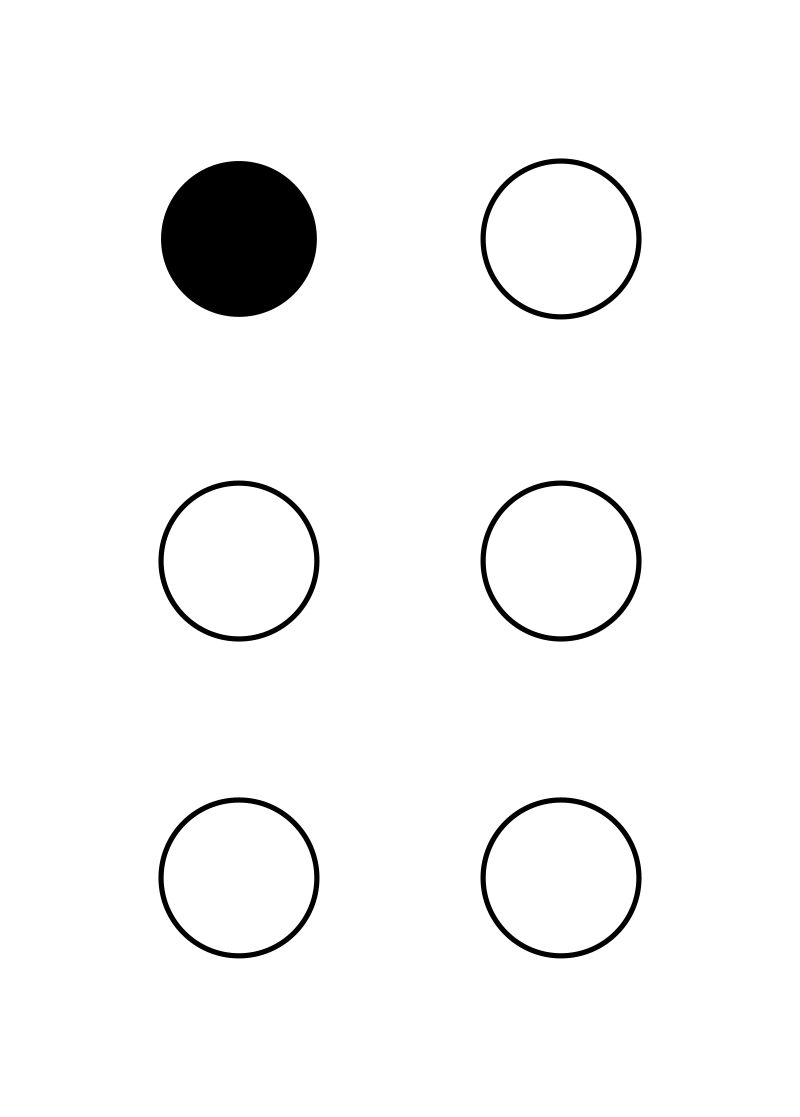
\includegraphics[width=\textwidth]{Braill_A.png}
	\end{minipage}
	\begin{minipage}{0.18\textwidth}
		\centering
		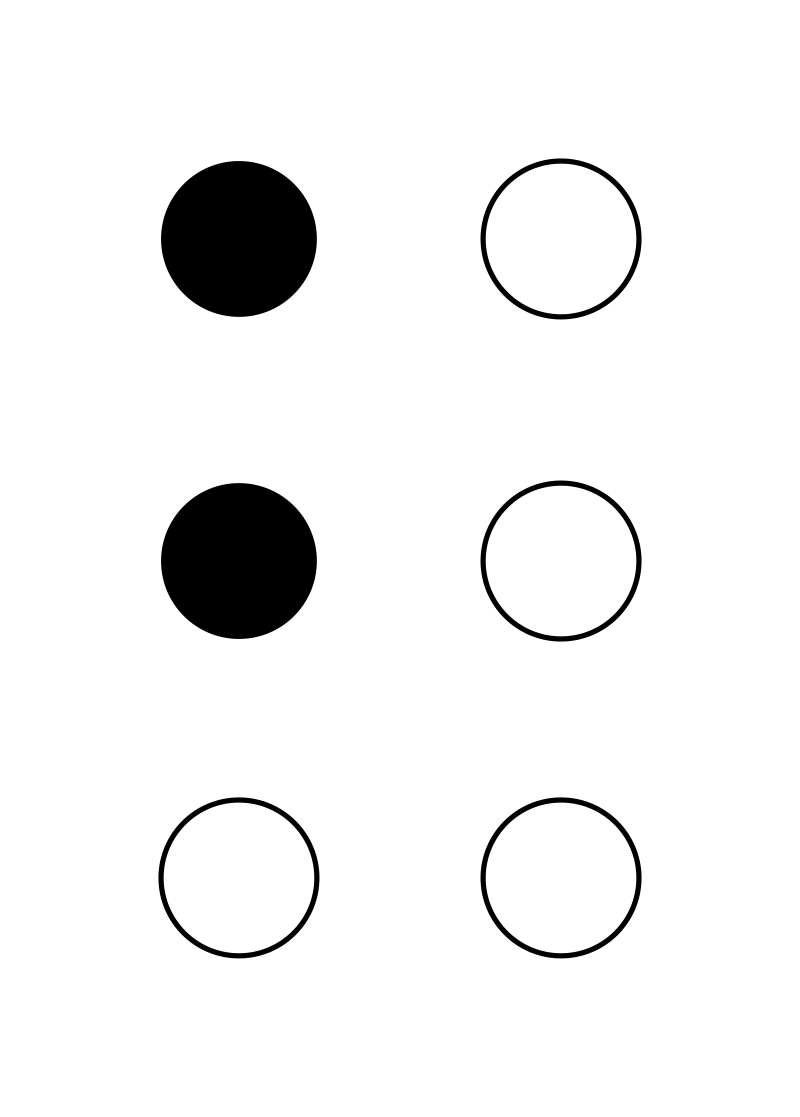
\includegraphics[width=\textwidth]{Braill_B.png}
	\end{minipage}
	\begin{minipage}{0.18\textwidth}
		\centering
		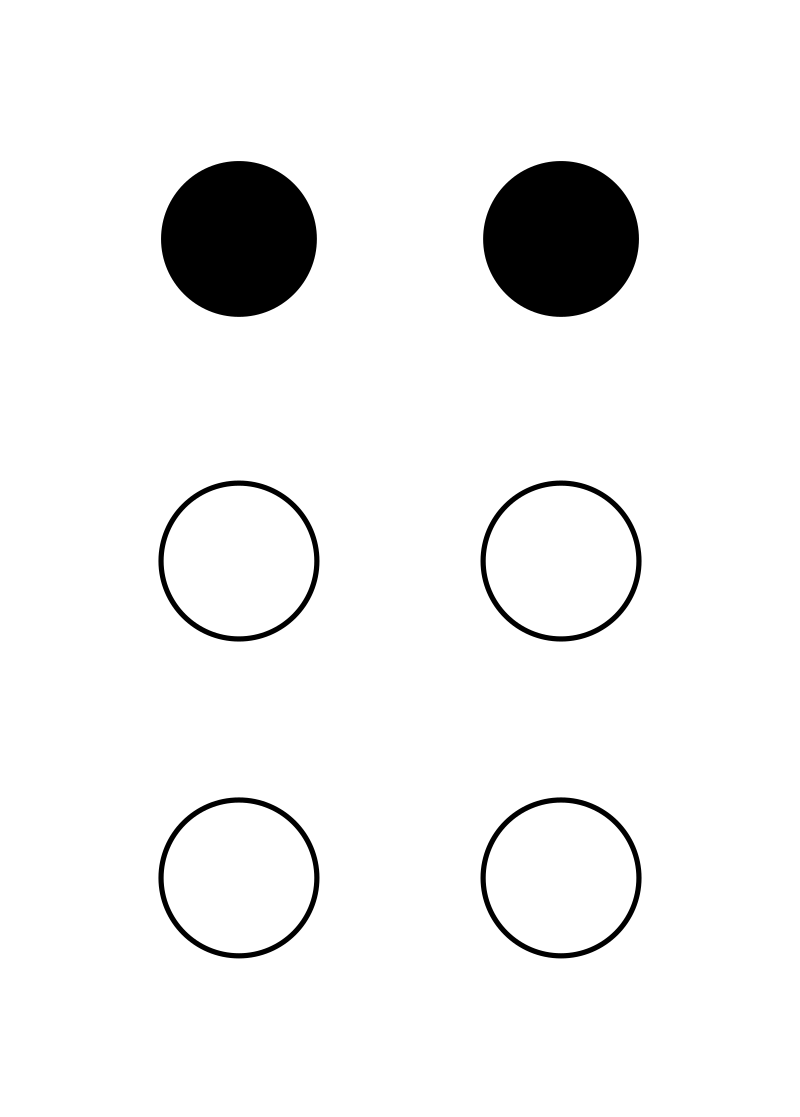
\includegraphics[width=\textwidth]{Braill_C.png}
	\end{minipage}
	\begin{minipage}{0.18\textwidth}
		\centering
		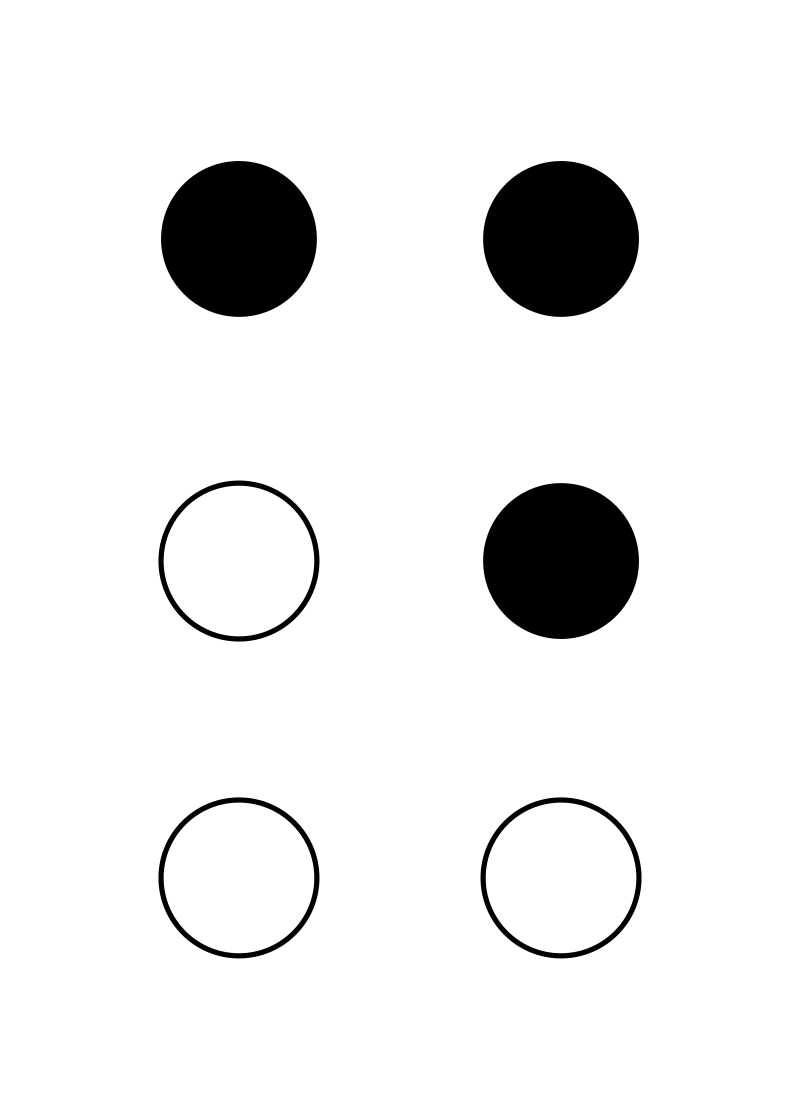
\includegraphics[width=\textwidth]{Braill_D.png}
	\end{minipage}\\
	Obliczyć, ile można utworzyć liter, korzystając z powyższego systemu.
}

\ZadanieTextowe{Obliczyć, ile jest różnych wyrazów, które można ułożyć z liter wyrazu \textbf{"STATUETKA"}.}

\ZadanieTextowe{Tata Michała to fanatyk wędkarstwa, a do tego bardzo niechlujny, przez co w domu zawsze są porozrzucane haczyki. Każdego dnia, gdy Michał wraca do domu, ma 70\% szans, że wbije sobie haczyk w nogę. Obliczyć prawdopodobieństwo, że w ciągu tygodnia roboczego (5 dni), wracając ze szkoły, wbije sobie haczyk przynajmniej raz.}

\ZadanieTextowe{Michał zrobił tacie awanturę po tym, jak w poprzednim tygodniu każdego dnia wbijał sobie haczyk w stopę. Tata zmienił swoje podejście, lecz tylko częściowo. Dalej pozostawia na podłodze haczyki, jednak jeśli Michał wbije sobie haczyk, to tata po sobie sprząta, a prawdopodobieństwo, że Michał wbije sobie haczyk, wynosi tylko 30\%. Obliczyć prawdopodobieństwo, że Michał wbije sobie haczyk dwa razy w przeciągu trzech dni (zakładając, że jego tata nie posprzątał po sobie wcześniej).}

\ZadanieTextowe{W 24-osobowej klasie pewien nauczyciel dał uczniom zadanie do rozwiązania. Niestety zrobiła je tylko połowa klasy, a druga połowa spisała je z Chatu GPT. Nauczyciel na następnej lekcji zamierza z tego zadania odpytać. Obliczyć prawdopodobieństwo, że przy losowym odpytaniu 3 osób nie trafi na osobę, która spisała zadanie od AI.}

\ZadanieTextowe{Do pewnej restauracji przyszła 8-osobowa grupa znajomych. Troje z nich zamówiło Kurczaka Gong Bao, dwoje Pierożki Xiu Mai, jedna osoba Rekina w czerwonym winie, a reszta Zupę z węgorza. Niestety zapominalski kelner nie zapamiętał, kto co zamówił. Obliczyć prawdopodobieństwo, że kelner dobrze rozda zamówione dania.}

\ZadanieTextowe{Dana jest próbka: $$5,6,2,2x,13,12,2,x,-4,2$$, której średnia arytmetyczna wynosi 5. Obliczyć wartość $x$.}

\Zadanie{Obliczyć medianę, dominantę i średnią arytmetyczną ocen testów studentów z wykresu.}{
	\centering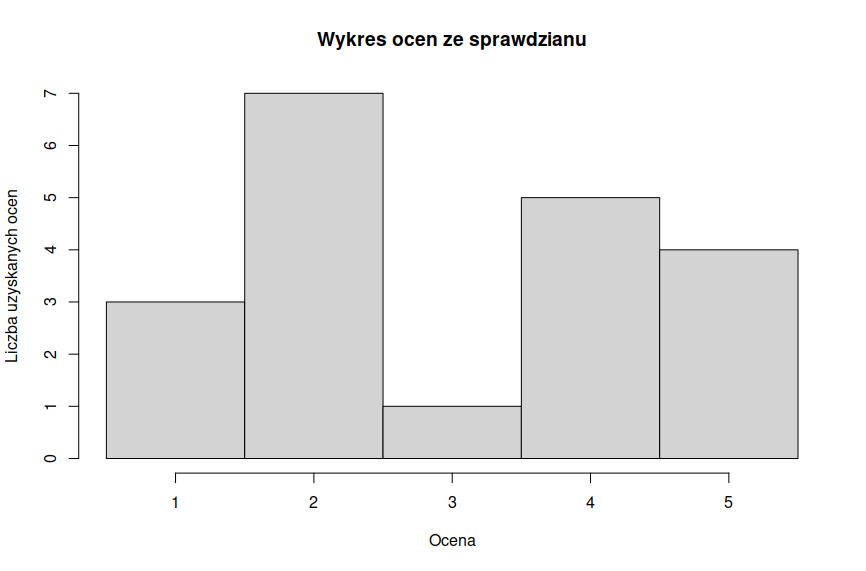
\includegraphics[scale=0.6]{Oceny.png}}
		
		
		



		\begin{center}
		
		\begin{tabular}{|c|c|c|c|c|c|c|c|c|c|c|}\hline
			Zadanie&1&2&3&4&5&6&7&8&9&10\\\hline
			Max&4&3&3&3&3&3&3&3&2&3\\\hline
			Punkty&&&&&&&&&&\\\hline
		\end{tabular}
	\end{center}
\end{document}
